\documentclass[12pt]{article}

\usepackage[margin=1in, left=0.6in, right=0.6in]{geometry}
\usepackage{fancyhdr} % header
\usepackage{hyperref} % links
\usepackage{amsmath,amsthm,amssymb} %math stuff
\usepackage{setspace} % increase line spacing
\usepackage[table]{xcolor} % align environment
% \usepackage{color, soul}
\usepackage{changepage} % for the adjustwidth environment
\usepackage{relsize} % Scaling the font
\usepackage{graphicx} \graphicspath{ {./images/} } % images
\usepackage{tabularx} % long tables
\usepackage{makecell} % newlines in a table cell
\usepackage{xfrac} % slanted fractions
\usepackage{stackengine} % for long division
\usepackage{scalerel} % for long division
\newcommand\showdiv[1]{\overline{\smash{\hstretch{.5}{)}\mkern-3.2mu\hstretch{.5}{)}}#1}}
\let\ph\phantom
% more long division
\usepackage{color,soul}

\definecolor{gray}{rgb}{0.5,0.5,0.5}

\setlength{\parindent}{0pt}
\everymath{\displaystyle}

\pagestyle{fancy}
\fancyhead[LO,L]{CSCD58 Assignment 2}
\fancyhead[CO,C]{Stephen Guo}
\fancyhead[RO,R]{1006313231}
\fancyfoot[LO,L]{}
\fancyfoot[CO,C]{\thepage}
\fancyfoot[RO,R]{}

\begin{document}
%----------------------------------------------------------------------------------
%                              Table of Contents
%----------------------------------------------------------------------------------
\begin{center}
	\hypertarget{toc}{\LARGE \underline{\textbf{Table of Contents}}}\\
\end{center}

\hyperlink{1}{\textbf{Question 1:}}
\vspace{1mm}
\hrule
~\\

\hyperlink{2}{\textbf{Question 2:}}
\vspace{1mm}
\hrule
~\\

{\textbf{Question 3:}}
\vspace{1mm}
\hrule
\vspace{1mm}
\hyperlink{3.1}{(a)}\\
\hyperlink{3.2}{(b)}\\
\hyperlink{3.3}{(c)}\\
\\

\hyperlink{4}{\textbf{Question 4:}}
\vspace{1mm}
\hrule
~\\

{\textbf{Question 5:}}
\vspace{1mm}
\hrule
\vspace{1mm}
\hyperlink{5.1}{(a)}\\
\hyperlink{5.2}{(b)}\\
~\\

{\textbf{Question 6:}}
\vspace{1mm}
\hrule
\vspace{1mm}
\hyperlink{6.1}{(1)}\\
\hyperlink{6.2}{(2)}\\
\hyperlink{6.3}{(3)}\\
\hyperlink{6.4}{(4)}\\
\hyperlink{6.5}{(5)}\\
\hyperlink{6.6}{(6)}\\
\hyperlink{6.7}{(7)}\\
\hyperlink{6.8}{(8)}\\
\hyperlink{6.9}{(9)}\\
~\\

{\textbf{Question 7:}}
\vspace{1mm}
\hrule
\vspace{1mm}
\hyperlink{7.1}{(1)}\\
\hyperlink{7.2}{(2)}\\
\\

\hyperlink{8}{\textbf{Question 8:}}
\vspace{1mm}
\hrule
~\\

\hyperlink{9}{\textbf{Question 9:}}
\vspace{1mm}
\hrule
~\\

\hyperlink{10}{\textbf{Question 10:}}
\vspace{1mm}
\hrule
~\\

{\textbf{Question 11:}}
\vspace{1mm}
\hrule
\vspace{1mm}
\hyperlink{11.1}{(a)}\\
\hyperlink{11.2}{(b)}\\
\hyperlink{11.3}{(c)}\\
\hyperlink{11.4}{(d)}\\
\hyperlink{11.5}{(e)}\\
\\

\hyperlink{12}{\textbf{Question 12:}}
\vspace{1mm}
\hrule
~\\

\newpage

%----------------------------------------------------------------------------------
%                                   Questions
%----------------------------------------------------------------------------------
\setstretch{1.2}
%----------------------------------------------------------------------------------
% !                                     1
%----------------------------------------------------------------------------------
\hyperlink{toc}{\hypertarget{1}{\LARGE \underline{\textbf{Question 1.}}}}\\
\begin{center}
	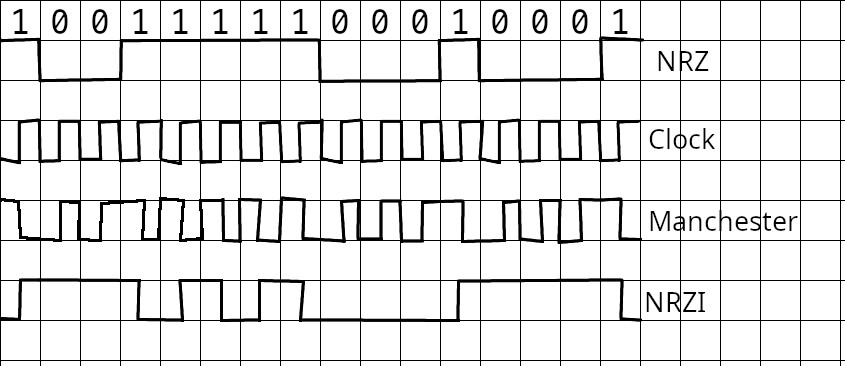
\includegraphics[width=\textwidth]{cscd58-a2-q1.jpg}
\end{center}
\newpage

%----------------------------------------------------------------------------------
% !                                     2
%----------------------------------------------------------------------------------
\hyperlink{toc}{\hypertarget{2}{\LARGE \underline{\textbf{Question 2.}}}}
\begin{verbatim}
1101  1110  1010  1101  1011  1110  1110  1111
turns into:
11011 11100 10110 11011 10111 11100 11100 11101
\end{verbatim}
\begin{center}
	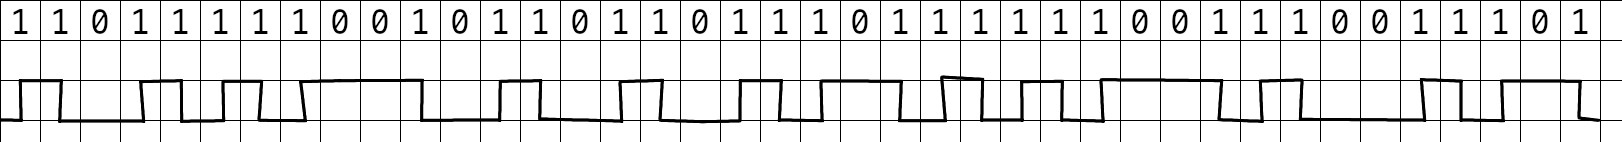
\includegraphics[width=\textwidth]{cscd58-a2-q2.jpg}
\end{center}
~\\

\newpage

%----------------------------------------------------------------------------------
% !                                     3
%----------------------------------------------------------------------------------
\hyperlink{toc}{\LARGE \underline{\textbf{Question 3.}}}\\
~\\\hyperlink{toc}{\hypertarget{3.1}{(a)}}
\begin{verbatim}
01111110 10100111 11111000 11110010 10011111 10111111 11100101
turns into:
011111010 10100111 110111000 11110010 100111110 101111101 11100101
\end{verbatim}
~\\\hyperlink{toc}{\hypertarget{3.2}{(b)}}\\
\begin{verbatim}
00111111 01110001 11110011 11111100 10101010 11001111 11100001
turns into:
001111101 01110001 111100011 111011100 10101010 11001111 101100001
\end{verbatim}

~\\\hyperlink{toc}{\hypertarget{3.3}{(c)}}\\
\begin{verbatim}
11111111 11111111 11111111 11111111 11111111 11111111 11111111
turns into:
111110111 1101111101 111101111 1011111011 111011111 0111110111 1101111101
\end{verbatim}
\newpage

%----------------------------------------------------------------------------------
% !                                     4
%----------------------------------------------------------------------------------
\hyperlink{toc}{\hypertarget{4}{\LARGE \underline{\textbf{Question 4.}}}}\\
\begin{verbatim}
011010111110101001111111011001111110
turns into:
01101011111101001111111011001111110
                      ^ error, there's 7 consecutive 1's
\end{verbatim}
\newpage

%----------------------------------------------------------------------------------
% !                                     5
%----------------------------------------------------------------------------------
\hyperlink{toc}{\LARGE \underline{\textbf{Question 5.}}}\\
~\\\hyperlink{toc}{\hypertarget{5.1}{(a)}}\\
% \(
% \stackunder{%
% 100000111 \stackon[1pt]{\showdiv{1011001001001011{00000000}}}{10101101100011{00}\ph{01001011}}% i don't get the last 2 0's
% }{%
% \Shortstack[l]{{\underline{100000111}\ph{011001001001011}}
% \ph{1 0}101110110 {\ph{10}\underline{100000111}}
% \ph{101 0}110111101 {\ph{1011}\underline{100000111}}
% \ph{10110}101101100 {\ph{10110}\underline{100000111}}
% \ph{101100 0}110010111 {\ph{1011001}\underline{100000111}}
% \ph{1011001 0}100100000 {\ph{10110010}\underline{100000111}}
% \ph{10110010 0000}110010000 {\ph{101100100100}\underline{100000111}}
% \ph{101100100 0000}100010010 {\ph{1011001001001}\underline{100000111}}
% \ph{1011001001 00000000}101100
% }
% }
% \)
% ~\\
%
% So the remainder is 101100, so we will subtract that from the message, or use logical XOR:
% \[
% 	\begin{array}{l@{\quad}cr@{}}
% 		 &        & 101100100100101100000000 \\
% 		 & \oplus & 101100                   \\ \cline{2-3}
% 		 &        & 101100100100101100101100
% 	\end{array}
% \]
% ~\\\\
% lolnvm
% ~\\\\
\(
\setstackgap{S}{1.5pt}
\stackMath\def\stackalignment{r}
\stackunder{%
100000111 \stackon[1pt]{\showdiv{101100100100101100000000}}{1011000101011101\ph{00000000}}% i don't get the last 2 0's
}{%
\Shortstack[l]{{\underline{100000111}\ph{100101100000000}}
\ph{00}1100011{10} \ph{00}\underline{100000111}
\ph{000}10001001{0} \ph{000}\underline{100000111}
\ph{0000000}10101{1011} \ph{0000000}\underline{100000111}
\ph{000000000}1011100{00} \ph{000000000}\underline{100000111}
\ph{00000000000}1110111{00} \ph{00000000000}\underline{100000111}
\ph{000000000000}11011011{0} \ph{000000000000}\underline{100000111}
\ph{0000000000000}10110001{0} \ph{0000000000000}\underline{100000111}
\ph{000000000000000}1100101{00} \ph{000000000000000}\underline{100000111}
\ph{0000000000000000}10010011
}
}
\)
~\\

So the remainder is 10010011, so we will subtract that from the message using logical XOR:
\[
	\begin{array}{l@{\quad}cr@{}}
		 &        & 101100100100101100000000 \\
		 & \oplus & 10010011                 \\ \cline{2-3}
		 &        & 101100100100101110010011
	\end{array}
\]
So the final message to send is: 101100100100101110010011

\newpage
\hyperlink{toc}{\hypertarget{5.2}{(b)}}\\
If the left most bit is inverted due to noise, then the new message will be: 001100100100101110010011

In that case, the long division will give us:\\

\(
\setstackgap{S}{1.5pt}
\stackMath\def\stackalignment{r}
\stackunder{%
100000111 \stackon[1pt]{\showdiv{001100100100101110010011}}{11001011010111\ph{00000000}}% i don't get the last 2 0's
}{%
\Shortstack[l]{{\underline{100000111}\ph{0101100000000}}
\ph{0}10010101{0} \ph{0}\underline{100000111}
\ph{0000}101101{101} \ph{0000}\underline{100000111}
\ph{000000}1101010{11} \ph{000000}\underline{100000111}
\ph{0000000}10101100{0} \ph{0000000}\underline{100000111}
\ph{000000000}1011111{01} \ph{000000000}\underline{100000111}
\ph{00000000000}1111010{00} \ph{00000000000}\underline{100000111}
\ph{000000000000}11101111{1} \ph{000000000000}\underline{100000111}
\ph{0000000000000}11011000{1} \ph{0000000000000}\underline{100000111}
\ph{00000000000000}10110110{}
}
}
\)
~\\\\

Which isn't a remainder of 0. This means that an error has occurred because the remainder of the message must be 0
\newpage

%----------------------------------------------------------------------------------
% !                                     6
%----------------------------------------------------------------------------------
\hyperlink{toc}{\LARGE \underline{\textbf{Question 6.}}}\\
~\\\hyperlink{toc}{\hypertarget{6.1}{(1)}}\\
\hl{0}011\hl{1}10\hl{0}\\[-2.5mm]
\hl{1}011\hl{0}10\hl{1}\\

So the hamming distance is 3

~\\\hyperlink{toc}{\hypertarget{6.2}{(2)}}\\
\begin{minipage}[t]{0.5\textwidth}
	\begin{center}
		$
			\begin{array}{l}
				\text{\hl{1}0\hl{1}\hl{1}\hl{0}1\hl{0}1} \\[-2.5mm]
				\text{\hl{0}0\hl{0}\hl{0}\hl{1}1\hl{1}1}
			\end{array}
		$ = Hamming distance 5
	\end{center}
\end{minipage}
\begin{minipage}[t]{0.5\textwidth}
	\begin{center}
		$
			\begin{array}{l}
				\text{\hl{1}\hl{0}\hl{1}10101} \\[-2.5mm]
				\text{\hl{0}\hl{1}\hl{0}10101}
			\end{array}
		$ = Hamming distance 3
	\end{center}
\end{minipage}\\

\begin{minipage}[t]{0.5\textwidth}
	\begin{center}
		$
			\begin{array}{l}
				\text{\hl{1}011\hl{0}10\hl{1}} \\[-2.5mm]
				\text{\hl{0}011\hl{1}10\hl{0}}
			\end{array}
		$ = Hamming distance 3
	\end{center}
\end{minipage}
\begin{minipage}[t]{0.5\textwidth}
	\begin{center}
		$
			\begin{array}{l}
				\text{10\hl{1}\hl{1}0\hl{1}0\hl{1}} \\[-2.5mm]
				\text{10\hl{0}\hl{0}0\hl{0}0\hl{0}}
			\end{array}
		$ = Hamming distance 4
	\end{center}
\end{minipage}\\

\begin{minipage}[t]{0.5\textwidth}
	\begin{center}
		$
			\begin{array}{l}
				\text{1\hl{0}1101\hl{0}1} \\[-2.5mm]
				\text{1\hl{1}1101\hl{1}1}
			\end{array}
		$ = Hamming distance 2
	\end{center}
\end{minipage}
\begin{minipage}[t]{0.5\textwidth}
	\begin{center}
		$
			\begin{array}{l}
				\text{1\hl{0}11\hl{0}1\hl{0}1} \\[-2.5mm]
				\text{1\hl{1}11\hl{1}1\hl{1}1}
			\end{array}
		$ = Hamming distance 3
	\end{center}
\end{minipage}\\

So the most likely transmitted codeword is 11110111
% 10110101

~\\\hyperlink{toc}{\hypertarget{6.3}{(3)}}\\
1, 10, 11, 100, 101, 110, 111, 1000, 1001, 1010, 1011\\
bit number 1, 2, 4, and 8 are parity bits\\
the rest are all data bits. \\

So we have 4 parity bits.
~\\\hyperlink{toc}{\hypertarget{6.4}{(4)}}\\
Total bits is 4 parity + 7 bits = 11 bits.

~\\\hyperlink{toc}{\hypertarget{6.5}{(5)}}\\
let $R$ be a redundant parity bit. Then the message would look like:
\begin{center}
	\texttt{1 0 1 R 1 0 0 R 1 R R}
\end{center}

\newpage
~\\\hyperlink{toc}{\hypertarget{6.6}{(6)}}\\
\[
	\underset{0001}{R1}\qquad
	\underset{0010}{R2}\qquad
	\underset{0011}{1} \qquad
	\underset{0100}{R3}\qquad
	\underset{0101}{0} \qquad
	\underset{0110}{0} \qquad
	\underset{0111}{1} \qquad
	\underset{1000}{R4}\qquad
	\underset{1001}{1} \qquad
	\underset{1010}{0} \qquad
	\underset{1011}{1} \qquad
\]\\
$R1 = 0$\\
\[
	\underset{0001}{0}\qquad
	\underset{0010}{R2}\qquad
	\underset{0011}{1} \qquad
	\underset{0100}{R3}\qquad
	\underset{0101}{0} \qquad
	\underset{0110}{0} \qquad
	\underset{0111}{1} \qquad
	\underset{1000}{R4}\qquad
	\underset{1001}{1} \qquad
	\underset{1010}{0} \qquad
	\underset{1011}{1} \qquad
\]\\
$R2 = 1$\\
\[
	\underset{0001}{0}\qquad
	\underset{0010}{1}\qquad
	\underset{0011}{1} \qquad
	\underset{0100}{R3}\qquad
	\underset{0101}{0} \qquad
	\underset{0110}{0} \qquad
	\underset{0111}{1} \qquad
	\underset{1000}{R4}\qquad
	\underset{1001}{1} \qquad
	\underset{1010}{0} \qquad
	\underset{1011}{1} \qquad
\]\\
$R3 = 1$\\
\[
	\underset{0001}{0}\qquad
	\underset{0010}{1}\qquad
	\underset{0011}{1} \qquad
	\underset{0100}{1}\qquad
	\underset{0101}{0} \qquad
	\underset{0110}{0} \qquad
	\underset{0111}{1} \qquad
	\underset{1000}{R4}\qquad
	\underset{1001}{1} \qquad
	\underset{1010}{0} \qquad
	\underset{1011}{1} \qquad
\]\\
$R4 = 0$\\
\[
	\underset{0001}{0}\qquad
	\underset{0010}{1}\qquad
	\underset{0011}{1} \qquad
	\underset{0100}{1}\qquad
	\underset{0101}{0} \qquad
	\underset{0110}{0} \qquad
	\underset{0111}{1} \qquad
	\underset{1000}{0}\qquad
	\underset{1001}{1} \qquad
	\underset{1010}{0} \qquad
	\underset{1011}{1} \qquad
\]\\

% $R1 = 1$\\
% $R2 = 0$\\
% $R3 = 0$\\
% $R4 = 1$\\

~\\\hyperlink{toc}{\hypertarget{6.7}{(7)}}\\
\begin{center}
	\texttt{1 0 1 0 1 0 0 1 1 1 0}
\end{center}

after tramsmission:
\begin{center}
	\texttt{1 0 1 0 1 1 0 1 1 1 0}
\end{center}

% 1 0 1 R 1 0 0 R 1 R R
~\\\hyperlink{toc}{\hypertarget{6.8}{(8)}}\\
\[
	\underset{0001}{R1}\qquad
	\underset{0010}{R2}\qquad
	\underset{0011}{1} \qquad
	\underset{0100}{R3}\qquad
	\underset{0101}{0} \qquad
	\underset{0110}{0} \qquad
	\underset{0111}{1} \qquad
	\underset{1000}{R4}\qquad
	\underset{1001}{1} \qquad
	\underset{1010}{0} \qquad
	\underset{1011}{1} \qquad
\]\\
turns to:
\[
	\underset{0001}{0}\qquad
	\underset{0010}{1}\qquad
	\underset{0011}{1} \qquad
	\underset{0100}{1}\qquad
	\underset{0101}{0} \qquad
	\underset{0110}{0} \qquad
	\underset{0111}{1} \qquad
	\underset{1000}{0}\qquad
	\underset{1001}{1} \qquad
	\underset{1010}{0} \qquad
	\underset{1011}{1} \qquad
\]\\

~\\\hyperlink{toc}{\hypertarget{6.9}{(9)}}\\
The redundant bits sequence is 0110, which is 6. It matches my expectations
since that's the bit that has been flipped.
\newpage

%----------------------------------------------------------------------------------
% !                                     7
%----------------------------------------------------------------------------------
\hyperlink{toc}{\LARGE \underline{\textbf{Question 7.}}}\\
~\\\hyperlink{toc}{\hypertarget{7.1}{(a)}}\\
% Expected bandwidth is just 8dB
\[
	\begin{array}{r@{}>{\displaystyle}l}
		\text{dB}                          & {} = 10 \times \log_{10} \left(\frac{S}{N}\right)    \\[6mm]
		20                                 & {} =  10 \times \log_{10} \left(\frac{S}{N}\right)   \\[6mm]
		\log_{10} \left(\frac{S}{N}\right) & {} = 2                                               \\[6mm]
		\frac{S}{N}                        & {} =                                             100 \\[6mm]
	\end{array}
\]~\\

\[
	\begin{array}{r@{}>{\displaystyle}l}
		C & {} = B \times \log_2 \left(1 + \frac{S}{N}\right) \\[6mm]
		  & {} = 16\ 000 \times \log_2 \left(1 + 100\right)   \\[6mm]
		  & {} = 16\ 000 \times \log_2 (101)                  \\[6mm]
		  & {} \approx 106\ 531.3837 \text{ bits/second}      \\[6mm]
	\end{array}
\]

~\\\hyperlink{toc}{\hypertarget{7.2}{(b)}}\\
\[
	\begin{array}{r@{}>{\displaystyle}l}
		C                                   & {} = B \times \log_2 \left(1 + \frac{S}{N}\right)           \\[6mm]
		50\ 000                             & {} = 1\ 000\ 000 \times \log_2 \left(1 + \frac{S}{N}\right) \\[6mm]
		\log_2 \left(1 + \frac{S}{N}\right) & {} = \frac{1}{20}                                           \\[6mm]
		1 + \frac{S}{N}                     & {} = 2^{\frac{1}{20}}                                       \\[6mm]
		\frac{S}{N}                         & {} = 2^\frac{1}{20} - 1                                     \\[6mm]
		                                    & {} \approx 0.035265                                         \\[6mm]
	\end{array}
\]

For the minimum signal-to-noise ratio, there is significantly more noise than signal.
% Noise stronger than signal?
\newpage

%----------------------------------------------------------------------------------
% !                                     8
%----------------------------------------------------------------------------------
\hyperlink{toc}{\hypertarget{8}{\LARGE \underline{\textbf{Question 8.}}}}\\
\begin{center}
	\begin{tabular}{|c|c|c|c|c|}
		\hline
		Band           & Range (Hz) & 10dB Capacity & 20dB Capacity & 30dB Capacity \\\hline
		\hline
		Narrowband     & 300-3400   & 10724.238018  & 20640.455597  & 30898.40140   \\\hline
		Wideband       & 50-7000    & 24043.04975   & 46274.56981   & 69272.22250   \\\hline
		Super-wideband & 50-14000   & 48259.07108   & 92882.05018   & 139042.80631  \\\hline
		Fullband       & 20-20000   & 69119.44374   & 133031.065425 & 199145.18065  \\\hline
	\end{tabular}
\end{center}

10dB
\begin{adjustwidth}{10mm}{}
	\[
		\begin{array}{r@{}>{\displaystyle}l}
			10 \text{dB}                       & {} = 10 \times \log_{10} \left(\frac{S}{N}\right) \\
			\log_{10} \left(\frac{S}{N}\right) & {} = 1                                            \\[6mm]
			\frac{S}{N}                        & {} = 10                                           \\
		\end{array}
	\]
\end{adjustwidth}~\\
for Narrowband
\begin{adjustwidth}{10mm}{}
	% $B = 3400 - 300 = 3100$\\
	% $\text{10} = 10 \times \log_{10} \left(\frac{S}{N}\right)$
	$
		\begin{array}{r@{}>{\displaystyle}l}
			B & {}= 3400 - 300 = 3100                       \\[2mm]
			C & {} = 3100 \times \log_2 (1 + 10)            \\
			  & {} \approx 10724.238018 \text{ bits/second} \\
		\end{array}
	$
\end{adjustwidth}~\\
for Wideband
\begin{adjustwidth}{10mm}{}
	$
		\begin{array}{r@{}>{\displaystyle}l}
			B & {}= 7000 - 50 = 6950                       \\[2mm]
			C & {} = 6950 \times \log_2 (1 + 10)           \\
			  & {} \approx 24043.04975 \text{ bits/second} \\
		\end{array}
	$
\end{adjustwidth}
for Super-wideband
\begin{adjustwidth}{10mm}{}
	$
		\begin{array}{r@{}>{\displaystyle}l}
			B & {}= 14000 - 50 = 13950                     \\[2mm]
			C & {} = 13950 \times \log_2 (1 + 10)          \\
			  & {} \approx 48259.07108 \text{ bits/second} \\
		\end{array}
	$
\end{adjustwidth}
for Fullband
\begin{adjustwidth}{10mm}{}
	$
		\begin{array}{r@{}>{\displaystyle}l}
			B & {}= 20000-20 = 19980                       \\[2mm]
			C & {} = 19980 \times \log_2 (1 + 10)          \\
			  & {} \approx 69119.44374 \text{ bits/second} \\
		\end{array}
	$
\end{adjustwidth}
\newpage
20dB
\begin{adjustwidth}{10mm}{}
	\[
		\begin{array}{r@{}>{\displaystyle}l}
			20 \text{dB}                       & {} = 10 \times \log_{10} \left(\frac{S}{N}\right) \\
			\log_{10} \left(\frac{S}{N}\right) & {} = 2                                            \\[6mm]
			\frac{S}{N}                        & {} = 100                                          \\
		\end{array}
	\]
\end{adjustwidth}~\\
for Narrowband
\begin{adjustwidth}{10mm}{}
	$
		\begin{array}{r@{}>{\displaystyle}l}
			B & {}= 3400 - 300 = 3100                       \\[2mm]
			C & {} = 3100 \times \log_2 (1 + 100)           \\
			  & {} \approx 20640.455597 \text{ bits/second} \\
		\end{array}
	$
\end{adjustwidth}~\\
for Wideband
\begin{adjustwidth}{10mm}{}
	$
		\begin{array}{r@{}>{\displaystyle}l}
			B & {}= 7000 - 50 = 6950                       \\[2mm]
			C & {} = 6950 \times \log_2 (1 + 100)          \\
			  & {} \approx 46274.56981 \text{ bits/second} \\
		\end{array}
	$
\end{adjustwidth}
for Super-wideband
\begin{adjustwidth}{10mm}{}
	$
		\begin{array}{r@{}>{\displaystyle}l}
			B & {}= 14000 - 50 = 13950                     \\[2mm]
			C & {} = 13950 \times \log_2 (1 + 100)         \\
			  & {} \approx 92882.05018 \text{ bits/second} \\
		\end{array}
	$
\end{adjustwidth}
for Fullband
\begin{adjustwidth}{10mm}{}
	$
		\begin{array}{r@{}>{\displaystyle}l}
			B & {}= 20000-20 = 19980                         \\[2mm]
			C & {} = 19980 \times \log_2 (1 + 100)           \\
			  & {} \approx 133031.065425 \text{ bits/second} \\
		\end{array}
	$
\end{adjustwidth}~\\


30dB
\begin{adjustwidth}{10mm}{}
	\[
		\begin{array}{r@{}>{\displaystyle}l}
			30 \text{dB}                       & {} = 10 \times \log_{10} \left(\frac{S}{N}\right) \\
			\log_{10} \left(\frac{S}{N}\right) & {} = 3                                            \\[6mm]
			\frac{S}{N}                        & {} = 1000                                         \\
		\end{array}
	\]
\end{adjustwidth}~\\
for Narrowband
\begin{adjustwidth}{10mm}{}
	$
		\begin{array}{r@{}>{\displaystyle}l}
			B & {}= 3400 - 300 = 3100                      \\[2mm]
			C & {} = 3100 \times \log_2 (1 + 1000)         \\
			  & {} \approx 30898.40140 \text{ bits/second} \\
		\end{array}
	$
\end{adjustwidth}~\\
for Wideband
\begin{adjustwidth}{10mm}{}
	$
		\begin{array}{r@{}>{\displaystyle}l}
			B & {}= 7000 - 50 = 6950                       \\[2mm]
			C & {} = 6950 \times \log_2 (1 + 1000)         \\
			  & {} \approx 69272.22250 \text{ bits/second} \\
		\end{array}
	$
\end{adjustwidth}
for Super-wideband
\begin{adjustwidth}{10mm}{}
	$
		\begin{array}{r@{}>{\displaystyle}l}
			B & {}= 14000 - 50 = 13950                      \\[2mm]
			C & {} = 13950 \times \log_2 (1 + 1000)         \\
			  & {} \approx 139042.80631 \text{ bits/second} \\
		\end{array}
	$
\end{adjustwidth}
for Fullband
\begin{adjustwidth}{10mm}{}
	$
		\begin{array}{r@{}>{\displaystyle}l}
			B & {}= 20000-20 = 19980                        \\[2mm]
			C & {} = 19980 \times \log_2 (1 + 1000)         \\
			  & {} \approx 199145.18065 \text{ bits/second} \\
		\end{array}
	$
\end{adjustwidth}
\newpage

%----------------------------------------------------------------------------------
% !                                     9
%----------------------------------------------------------------------------------
\hyperlink{toc}{\hypertarget{9}{\LARGE \underline{\textbf{Question 9.}}}}\\
% ~\\\hyperlink{toc}{\hypertarget{9.1}{(a)}}\\
Let blank cell = distance $\infty$\\

\begin{center}
	\begin{tabular}{|c||c|c|c|c|c|c|}
		\hline
		  & A & B & C & D & E & F \\\hline
		\hline
		A & 0 & 2 &   & 5 &   &   \\\hline
		B & 2 & 0 & 2 &   & 1 &   \\\hline
		C &   & 2 & 0 & 2 &   & 3 \\\hline
		D & 5 &   & 2 & 0 &   &   \\\hline
		E &   & 1 &   &   & 0 & 3 \\\hline
		F &   &   & 3 &   & 3 & 0 \\\hline
	\end{tabular}
\end{center}
A:\\
\begin{tabular}{|c|c|c|}
	\hline
	Destination & Cost & NextHop \\\hline
	\hline
	B           & 2    & B       \\\hline
	C           &      &         \\\hline
	D           & 5    & D       \\\hline
	E           &      &         \\\hline
	F           &      &         \\\hline
\end{tabular}
\begin{tabular}{|c|c|c|}
	\hline
	Destination & Cost & NextHop \\\hline
	\hline
	B           & 2    & B       \\\hline
	C           & 4    & B       \\\hline
	D           & 5    & D       \\\hline
	E           & 3    & B       \\\hline
	F           &      &         \\\hline
\end{tabular}
\begin{tabular}{|c|c|c|}
	\hline
	Destination & Cost & NextHop \\\hline
	\hline
	B           & 2    & B       \\\hline
	C           & 4    & B       \\\hline
	D           & 5    & D       \\\hline
	E           & 3    & B       \\\hline
	F           & 6    & E       \\\hline
\end{tabular}

B:\\
\begin{tabular}{|c|c|c|}
	\hline
	Destination & Cost & NextHop \\\hline
	\hline
	A           & 2    & A       \\\hline
	C           & 2    & C       \\\hline
	D           &      &         \\\hline
	E           & 1    & E       \\\hline
	F           &      &         \\\hline
\end{tabular}
\begin{tabular}{|c|c|c|}
	\hline
	Destination & Cost & NextHop \\\hline
	\hline
	A           & 2    & A       \\\hline
	C           & 2    & C       \\\hline
	D           & 4    & C       \\\hline
	E           & 1    & E       \\\hline
	F           & 4    & E       \\\hline
\end{tabular}
\begin{tabular}{|c|c|c|}
	\hline
	Destination & Cost & NextHop \\\hline
	\hline
	A           & 2    & A       \\\hline
	C           & 2    & C       \\\hline
	D           & 4    & C       \\\hline
	E           & 1    & E       \\\hline
	F           & 4    & E       \\\hline
\end{tabular}\\[3mm]

C:\\
\begin{tabular}{|c|c|c|}
	\hline
	Destination & Cost & NextHop \\\hline
	\hline
	A           &      &         \\\hline
	B           & 2    & B       \\\hline
	D           & 2    & D       \\\hline
	E           &      &         \\\hline
	F           & 3    & F       \\\hline
\end{tabular}
\begin{tabular}{|c|c|c|}
	\hline
	Destination & Cost & NextHop \\\hline
	\hline
	A           & 4    & B       \\\hline
	B           & 2    & B       \\\hline
	D           & 2    & D       \\\hline
	E           & 3    & B       \\\hline
	F           & 3    & F       \\\hline
\end{tabular}
\begin{tabular}{|c|c|c|}
	\hline
	Destination & Cost & NextHop \\\hline
	\hline
	A           & 4    & B       \\\hline
	B           & 2    & B       \\\hline
	D           & 2    & D       \\\hline
	E           & 3    & B       \\\hline
	F           & 3    & F       \\\hline
\end{tabular}\\[3mm]

D:\\
\begin{tabular}{|c|c|c|}
	\hline
	Destination & Cost & NextHop \\\hline
	\hline
	A           & 5    & A       \\\hline
	B           &      &         \\\hline
	C           & 2    & C       \\\hline
	E           &      &         \\\hline
	F           &      &         \\\hline
\end{tabular}
\begin{tabular}{|c|c|c|}
	\hline
	Destination & Cost & NextHop \\\hline
	\hline
	A           & 5    & A       \\\hline
	B           & 4    & C       \\\hline
	C           & 2    & C       \\\hline
	E           &      &         \\\hline
	F           & 5    & C       \\\hline
\end{tabular}
\begin{tabular}{|c|c|c|}
	\hline
	Destination & Cost & NextHop \\\hline
	\hline
	A           & 5    & A       \\\hline
	B           & 4    & C       \\\hline
	C           & 2    & C       \\\hline
	E           & 5    & C       \\\hline
	F           & 5    & C       \\\hline
\end{tabular}\\[3mm]

E:\\
\begin{tabular}{|c|c|c|}
	\hline
	Destination & Cost & NextHop \\\hline
	\hline
	A           &      &         \\\hline
	B           & 1    & B       \\\hline
	C           &      &         \\\hline
	D           &      &         \\\hline
	F           & 3    & F       \\\hline
\end{tabular}
\begin{tabular}{|c|c|c|}
	\hline
	Destination & Cost & NextHop \\\hline
	\hline
	A           & 3    & B       \\\hline
	B           & 1    & B       \\\hline
	C           & 3    & B       \\\hline
	D           &      &         \\\hline
	F           & 3    & F       \\\hline
\end{tabular}
\begin{tabular}{|c|c|c|}
	\hline
	Destination & Cost & NextHop \\\hline
	\hline
	A           & 3    & B       \\\hline
	B           & 1    & B       \\\hline
	C           & 3    & B       \\\hline
	D           & 5    & C       \\\hline
	F           & 3    & F       \\\hline
\end{tabular}

F:\\
\begin{tabular}{|c|c|c|}
	\hline
	Destination & Cost & NextHop \\\hline
	\hline
	A           &      &         \\\hline
	B           &      &         \\\hline
	C           & 3    & C       \\\hline
	D           &      &         \\\hline
	E           & 3    & E       \\\hline
\end{tabular}
\begin{tabular}{|c|c|c|}
	\hline
	Destination & Cost & NextHop \\\hline
	\hline
	A           &      &         \\\hline
	B           & 4    & E       \\\hline
	C           & 3    & C       \\\hline
	D           & 5    & C       \\\hline
	E           & 3    & E       \\\hline
\end{tabular}
\begin{tabular}{|c|c|c|}
	\hline
	Destination & Cost & NextHop \\\hline
	\hline
	A           & 6    & B       \\\hline
	B           & 4    & E       \\\hline
	C           & 3    & C       \\\hline
	D           & 5    & C       \\\hline
	E           & 3    & E       \\\hline
\end{tabular}\\[3mm]

% ~\\\hyperlink{toc}{\hypertarget{9.2}{(b)}}\\
\begin{center}
	\begin{tabular}{|c||c|c|c|c|c|c|c|}
		\hline
		  & A & B & C & D & E & F \\\hline
		\hline
		A & 0 & 2 & 4 & 5 & 3 & 6 \\\hline
		B & 2 & 0 & 2 & 4 & 1 & 4 \\\hline
		C & 4 & 2 & 0 & 2 & 3 & 3 \\\hline
		D & 5 & 4 & 2 & 0 & 5 & 5 \\\hline
		E & 3 & 1 & 3 & 5 & 0 & 3 \\\hline
		F & 6 & 4 & 3 & 5 & 3 & 0 \\\hline
	\end{tabular}
\end{center}
% A:\\
% \begin{tabular}{|c|c|c|}
% 	\hline
% 	Destination & Cost & NextHop \\\hline
% 	\hline
% 	B           & 2    & B       \\\hline
% 	C           & 4    & B       \\\hline
% 	D           & 5    & D       \\\hline
% 	E           & 3    & B       \\\hline
% 	F           &      &         \\\hline
% \end{tabular}\\[3mm]
%
% B:\\
% \begin{tabular}{|c|c|c|}
% 	\hline
% 	Destination & Cost & NextHop \\\hline
% 	\hline
% 	A           & 2    & A       \\\hline
% 	C           & 2    & C       \\\hline
% 	D           &      &         \\\hline
% 	E           & 1    & E       \\\hline
% 	F           &      &         \\\hline
% \end{tabular}\\[3mm]
%
% C:\\
% \begin{tabular}{|c|c|c|}
% 	\hline
% 	Destination & Cost & NextHop \\\hline
% 	\hline
% 	A           &      &         \\\hline
% 	B           & 2    & B       \\\hline
% 	D           & 2    & D       \\\hline
% 	E           &      &         \\\hline
% 	F           & 3    & F       \\\hline
% \end{tabular}\\[3mm]
%
% D:\\
% \begin{tabular}{|c|c|c|}
% 	\hline
% 	Destination & Cost & NextHop \\\hline
% 	\hline
% 	A           & 5    & A       \\\hline
% 	B           &      &         \\\hline
% 	C           & 2    & C       \\\hline
% 	E           &      &         \\\hline
% 	F           &      &         \\\hline
% \end{tabular}\\[3mm]
%
% E:\\
% \begin{tabular}{|c|c|c|}
% 	\hline
% 	Destination & Cost & NextHop \\\hline
% 	\hline
% 	A           &      &         \\\hline
% 	B           & 1    & B       \\\hline
% 	C           &      &         \\\hline
% 	D           &      &         \\\hline
% 	F           & 3    & F       \\\hline
% \end{tabular}\\[3mm]
%
% F:\\
% \begin{tabular}{|c|c|c|}
% 	\hline
% 	Destination & Cost & NextHop \\\hline
% 	\hline
% 	A           &      &         \\\hline
% 	B           &      &         \\\hline
% 	C           & 3    &         \\\hline
% 	D           &      &         \\\hline
% 	E           & 3    &         \\\hline
% \end{tabular}\\[3mm]

% ~\\\hyperlink{toc}{\hypertarget{9.3}{(c)}}\\
\newpage

%----------------------------------------------------------------------------------
% !                                     10
%----------------------------------------------------------------------------------
\hyperlink{toc}{\hypertarget{10}{\LARGE \underline{\textbf{Question 10.}}}}\\
\begin{center}
	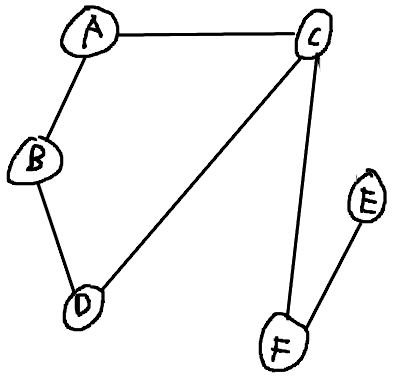
\includegraphics[width=\textwidth]{cscd58-a2-q10.png}
\end{center}
\newpage

%----------------------------------------------------------------------------------
% !                                     11
%----------------------------------------------------------------------------------
\hyperlink{toc}{\LARGE \underline{\textbf{Question 11.}}}\\
~\\\hyperlink{toc}{\hypertarget{11.1}{(a)}}\\
\texttt{128.96.171.92 AND 255.255.254.0 = 128.96.170.0}\\
\texttt{128.96.171.92 AND 255.255.252.0 = 128.96.168.0}\\
So it sends the packet to Interface 0\\

~\\\hyperlink{toc}{\hypertarget{11.2}{(b)}}\\
\texttt{128.96.167.151 AND 255.255.254.0 = 128.96.166.0}\\
\texttt{128.96.167.151 AND 255.255.252.0 = 128.96.164.0}\\
So it sends the packet to R2\\

% 254 = 11111110

~\\\hyperlink{toc}{\hypertarget{11.3}{(c)}}\\
\texttt{128.96.163.151 AND 255.255.254.0 = 128.96.162.0}\\
\texttt{128.96.163.151 AND 255.255.252.0 = 128.96.160.0}\\
So it sends the packet to R4 (no match)\\

~\\\hyperlink{toc}{\hypertarget{11.4}{(d)}}\\
\texttt{128.96.169.192 AND 255.255.254.0 = 128.96.168.0}\\
\texttt{128.96.169.192 AND 255.255.252.0 = 128.96.168.0}\\
So it sends the packet to Interface 1\\

~\\\hyperlink{toc}{\hypertarget{11.5}{(e)}}\\
\texttt{128.96.165.121 AND 255.255.254.0 = 128.96.164.0}\\
\texttt{128.96.165.121 AND 255.255.252.0 = 128.96.164.0}\\
So it sends the packet to R3
\newpage

%----------------------------------------------------------------------------------
% !                                     12
%----------------------------------------------------------------------------------
\hyperlink{toc}{\hypertarget{12}{\LARGE \underline{\textbf{Question 12.}}}}\\
\begin{center}
	\begin{tabular}{|c|l|l|}
		\hline
		Step & Confirmed                               & Tentative       \\\hline
		\hline
		1    & (A,0,-)                                 &                 \\\hline
		2    & (A,0,-)                                 & (B,1,B) (D,5,D) \\\hline
		3    & (A,0,-) (B,1,B)                         & (D,5,D)         \\\hline
		4    & (A,0,-) (B,1,B)                         & (D,4,B) (C,5,D) \\\hline
		5    & (A,0,-) (B,1,B) (D,4,B)                 & (C,5,D)         \\\hline
		6    & (A,0,-) (B,1,B) (D,4,B) (C,5,D)         & (C,5,D) (E,6,C) \\\hline
		7    & (A,0,-) (B,1,B) (D,4,B) (C,5,D)         & (E,6,C)         \\\hline
		8    & (A,0,-) (B,1,B) (D,4,B) (C,5,D) (E,6,C) &                 \\\hline
	\end{tabular}
\end{center}
\end{document}
